\subsection{Thoughts about the map}
In the original idea, we number the location and record the intensity to form the map from one end of the channel to the other end. This is wrong because this kind of map measures the diffusion part of the mixing much more than the stirring part of it. The hint here is that when we number the location, we lose the information of the geometric relations between cells, which can be very important in stirring effect.

On the other hand, the mixing rate of a Markov chain, which can be represented by the SLEM of it, is well studied, so we really want to keep the map being Markov. The way to go is to re-define the Markov process.

From the mistakes we made and from the properties of a Markov process, it suggests the following things: 

\begin{itemize}
\item We need to "number" the unimportant things and "record" the important ones.    
\item The map has to be linear.
\item $x$ has to be a distribution.
\item The final distribution can be predicted by simulating the Markov process.
\item The initial distribution can be understood by veiwing $x$.
\end{itemize} 

An idea is to number the frequency and to record the energy or the intensity that concentrates in a certain frequency. In the initial distribution, the energy must concentrate in low frequencies and hopefully in the steady state distribution the energy moves to high frequencies or evenly distributes in all frequencies. 
Hence in this formulation, not only we want to minimize the SLEM to accelerate the mixing, but also we indicate a certain final distribution $\pi$. This can be achieved by applying the method suggested by S. Boyd (not sure).
 
Here are the steps,
\begin{itemize}
\item We have to first define the distribution which has the above properties.
\item It can be evaluated when the certain red/blue distribution is given.
\item It can be also evaluated when only the map is given. 
\item The Markov matrix has to be very sparse. 
\end{itemize} 

Note about the sparsity: we can assume the energy in a certain frequency generally only transfers to its neighboring frequencies. 

\subsection{An Example}
In this section we use a simplified 2-D flow model to demonstrate how a suitable Markov chain is built to simulate the mixing process. This model is so simple that it lacks some of the properties that a 3-D flow can have, but it is sufficient for our use.
Let us consider the 2-D flow shown in figure 1. The ends of the channel are divided into three equal-sized grid cells with area $a$ and numbered as 1, 2 and 3 from top to bottom. The liquid to be mix are injected from the left end of this channel and flows out from the right end of it. The average normal velocity at each cell at both ends are named as $v^{k}$ and $v^{k+1} \in \mathbb{R}^3$. Let us further assume the flow is compressible and has average densities $\rho^{k}$ and $\rho^{k+1} \in \mathbb{R}^3$ at the left and the right ends respectively. Then the mass flow rates at both ends are $\dot{m}_i^{k} = v^{k}_i \rho^{k}_i a$ and  $\dot{m}_i^{k+1} = v^{k+1}_i \rho^{k+1}_i a$ for all $i$, and we have
   $$\mathbf{1}^T\dot{m}^{k}=\mathbf{1}^T\dot{m}^{k+1} $$ 


Suppose the flow is dyed red at each cell with some solution with intensities $\mu^{k}_i\in [0,1]$, for $i \in \{1,2,3\}$ at the left end, then $\mu^{k}_i$ is the "color" of the flow at each cell. Hence it is also the property we need to evaluate the mixing rate or mix-norm. Let $x_i^{k} = \mu_i^{k} \times \dot{m}_i^{k}$ for $i \in \{1,2,3\}$. $x^{k}$ is obviously the mass flow rate of the solution going into the channel. This leads to another equality,
  $$\mathbf{1}^T x^{k} =\mathbf{1}^T x^{k+1} $$ 

Suppose inside the channel there is some mechanism that steers the streamlines. Three of them are plotted on the figure. Then we have the following relations,
\begin{eqnarray*}
 x^{k+1} = A^T x^k, &  \mu^{k+1} = B \mu^{k} \\  \mbox{where  }
 A = \left[\begin{matrix}
        1 & 0 & 0 \\
        1 & 0 & 0 \\
        0 & 2/3 & 1/3\\ 
     \end{matrix}\right], & 
 B = \left[\begin{matrix}
        2/3 & 1/3 & 0 \\
        0 & 0 & 1 \\
        0 & 0 & 1\\ 
     \end{matrix}\right]
\end{eqnarray*}
One needs to be careful about how we get these two matrices. For matrix $A$, it decides how much proportion of the flow at cell $i$ goes to cell $j$. This means we need only to use streamlines $2$ and $3$. Streamline $1$ is unrelated. As for matrix $B$, it decides how the flow from cell $i$ is weighted at cell $j$, so strealmlines $1$ and $2$ are necessary, whereas $3$ is unrelated. 

This result tells us that we can either integrate the streamline forward in time from the boundries between cell $i$s to get matrix $B$, which transits the "color", or do it backward in time from the boundries between cell $j$s to get matrix $A$, which transits the mass flow rate of the solution. 

It also becomes clear that none of $A$ or $B$ contains all the information provided by the velocity/density field. In fact, $A$ and $B$ are related by
$$ B_{ij}{\dot{m}_i^{k+1}} = A_{ji} {\dot{m}_j^k} \mbox{  for all } i,j \in \{1,2,3\}$$

The above equation states that to get $B$ from $A$, we first unload the right end mass flow rate information and then equip with the left end one. 

Although it seems to be, state transition matrices $A$ and $B$ are actually indifferent for compressible or incompressible flows as long as the streamlines are given. For imcompressible flow, one can simply chage the mass flow rate $\dot{m}_i$ to the velocity $v_i$ because the cells are equal-sized.  

To furnish this example, let us now consider a 3-D periodical incompressible flow. The only difference is now the velocities $v^{k}_i = v^{k+1}_i= v_i$ for all $i$. Hence we have
$$ v = A^T v$$
i.e. $v$ is a left eigenvector of $A$. 
If we reverse the flow direction, the states then transit by
$$ x^k = B^T x^{k+1} , \mu^k = A \mu^{k+1}$$
Which says $v$ is also a left eigenvector of $B$ because $-v$ is the solution of the reversed flow. One should also keep in mind that both $A$ and $B$ have an right eigenvector $\mathbf{1}$.
  

Here are the details about $A$ and $B$
\begin{itemize}
\item $A_{ij}$ : flow forward, the proportion of cell $i$ going to cell $j$.\\
\item $A_{ij}$ : flow backward, the proportion of cell $i$ coming from cell $j$.\\
\item $B_{ij}$ : flow backward, the proportion  cell $i$ going to cell $j$. \\
\item $B_{ij}$ : flow forward, the proportion of cell $i$ coming from cell $j$. 
\end{itemize}

%%%%%%%%%%%%%%%%%%%%%%%%%%%%%%%%%%%%%%%%%%%%%%%%%%%%%%%%%%%%%%%%%%%%%%%%%%%%%%%%%%%%%%%%%
%%%%%%%%%%%%%%%%%%%%%%%%%%%%%%%%%%%%%%%%%%%%%%%%%%%%%%%%%%%%%%%%%%%%%%%%%%%%%%%%%%%%%%%%%
   Suppose $\mathbf{M}_1 v_2 = \lambda_{2}(\mathbf{M}_1)v_2$, i.e., $v_2$ is the eigenvector of $\mathbf{M}_1$ with respect to $\lambda_{2}$. Here we prove $v_2 \otimes \mathbf{1}$ is an eigenvector of $\mathbf{M}_2$ with eigenvalue $1-\frac{4\pi^{2}b}{2n^2}$.
\begin{eqnarray*}
  \mathbf{M}_2 (v_2 \otimes \mathbf{1}) &=& \frac{1}{2}\left( \mathbf{M}_{1}\otimes\mathbf{I}+ 
                                            \mathbf{I}\otimes \mathbf{M}_{1} \right)( v_2 \otimes \mathbf{1}) \\
                                        &=& \frac{1}{2}(\mathbf{M}_{1}\otimes\mathbf{I}) (v_2 \otimes \mathbf{1})+
                                            \frac{1}{2}(\mathbf{I}\otimes \mathbf{M}_{1}) (v_2 \otimes \mathbf{1})\\
                                        &=& \frac{1}{2}(\mathbf{M}_{1} v_2)\otimes(\mathbf{I} \mathbf{1}) +
                                            \frac{1}{2}(\mathbf{I} v_2)\otimes(\mathbf{M}_{1} \mathbf{1})\\
                                        &=& \frac{1}{2}(\lambda_{2}(\mathbf{M}_1) v_2 \otimes \mathbf{1}) +
                                            \frac{1}{2}( v_2 \otimes \mathbf{1})\\
                                        &=& \frac{1}{2}(\lambda_{2}(\mathbf{M}_1)+1)( v_2 \otimes \mathbf{1})
\end{eqnarray*}
Hence $\frac{1}{2}(\lambda_{2}(\mathbf{M}_1)+1)$ is an eigenvalue of $\mathbf{M}_2$. In the above derivation, we use the fact $ (A \otimes B)(x \otimes y) = Ax \otimes By $ for any $A,B,x,y$ with correct dimensions. In realizing that $\frac{1}{2}(\lambda_{2}(\mathbf{M}_1)+1)$ is actually the second largest eigenvalue of $\mathbf{M}_2$,

%%%%%%%%%%%%%%%%%%%%%%%%%%%%%%%%%%%%%%%%%%%%%%%%%%%%%%%%%%%%%%%%%%%%%%%%%%%%%%%%%%%%%%%%%%%
%%%%%%%%%%%%%%%%%%%%%%%%%%%%%%%%%%%%%%%%%%%%%%%%%%%%%%%%%%%%%%%%%%%%%%%%%%%%%%%%%%%%%%%%%%%%


First we define a 1-D diffusion matrix
$\mathbf{M}_{1}\in\mathbb{R}^{n\times n}$ to be
\begin{eqnarray*}
  \mathbf{M}_{1} =  \left[
             \begin{matrix}
               1-2b & b & 0   & ...  &    &  b \\
               b & 1-2b & b   & ...  &    &    \\
               0 & b & 1-2b   & b    &    &    \\
                 &   &     &      & \ddots & \\
               b & ... &     &    & b  &  a \\
             \end{matrix}
           \right]
\end{eqnarray*}
 The second largest eigenvalue
of $\mathbf{M}_{1}$ can be easily derived
\begin{eqnarray*}
 \lim_{n\to\infty}\lambda_{2}(M_1) = 1-\frac{4\pi^{2}b}{n^2}
\end{eqnarray*}

We choose the 2-D diffusion matrix to be
$M_{2}\in\mathbb{R}^{n^{2}\times n^{2}}$
\begin{eqnarray*}
 M_{2} = \frac{1}{2}\left( M_{1}\otimes I+ I\otimes M_{1} \right)
\end{eqnarray*}
where $I$ is the identity matrix which has the same size as $M_{1}$
and $\otimes$ refers to Kronecker product. One can easily prove that
the spectral gap of $M_2$ is $1- \frac{1}{2}(\lambda_{2}(M_1)+1) =
\frac{1}{2}(1-\lambda_{2}(M_1))$.

This is of course just one choice of the 2-D diffusion matrix. For a
given diffusibility $k$ and $\triangle t$, we can calculat $b$ as
\begin{eqnarray*}
b = \frac{n^2}{2\pi^2}(1-e^{-4\pi^2 k \triangle t})
\end{eqnarray*}
Since $b < 0.5$ is the necessary condition for $M$ to be positive, the above expression can not be applied if $k$ and $\triangle t$ are too large. In this case, one can always use a small $\triangle t$ and the equality $M^p(k,\triangle t) = M(k,p \triangle t)$ for any $p \in \mathbb{N}$ to create a suitable $M$.


%%%%%%%%%%%%%%%%%%%%%%%%%%%%%%%%%%%%%%%%%%%%%%%%%%%%%%%%%%%%%%%%%%%%%%%%%%%%%%%%%%%%

\subsection{Long-time Behavior}

Standard Map with $\epsilon = 0.1$, $k$ varies from $0$ to $0.07$. Initial condition $cos(2\pi x)$

\centerline{\scalebox{0.5}[0.5]{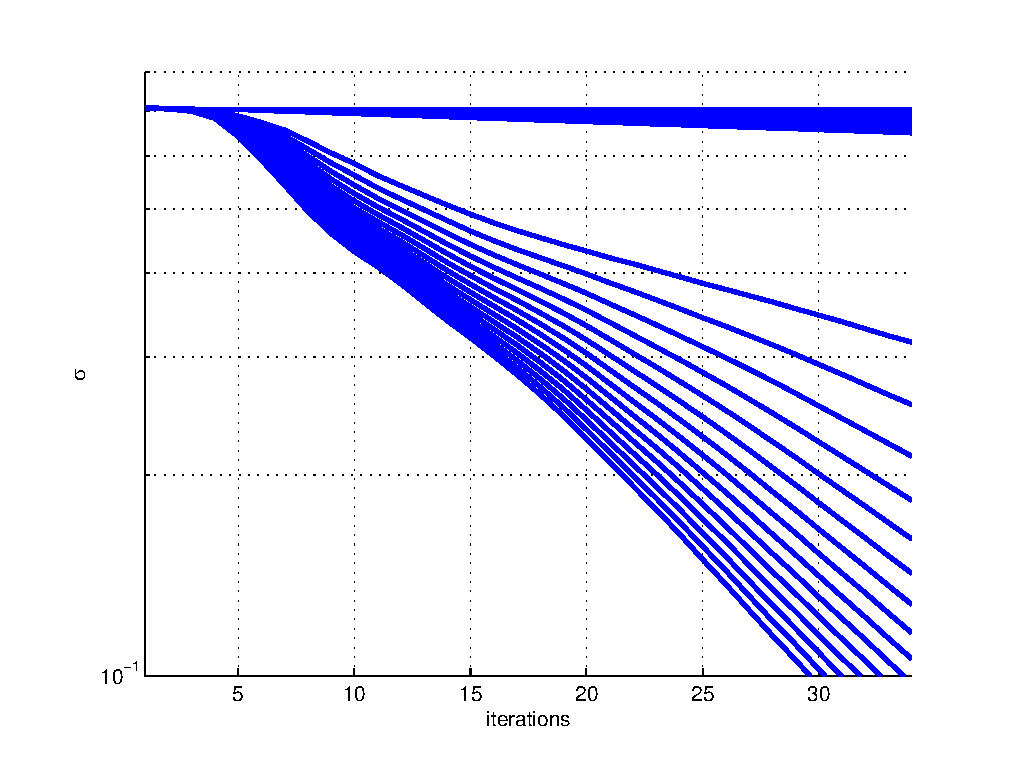
\includegraphics{standardmap_epsilon_0.2_sigma_compare.eps}}}

We measure the slope of each curve for the last $20$ points. From the slope an equivalent $k$ is calculated. The result is plotted in the following figure.





\centerline{\scalebox{0.5}[0.5]{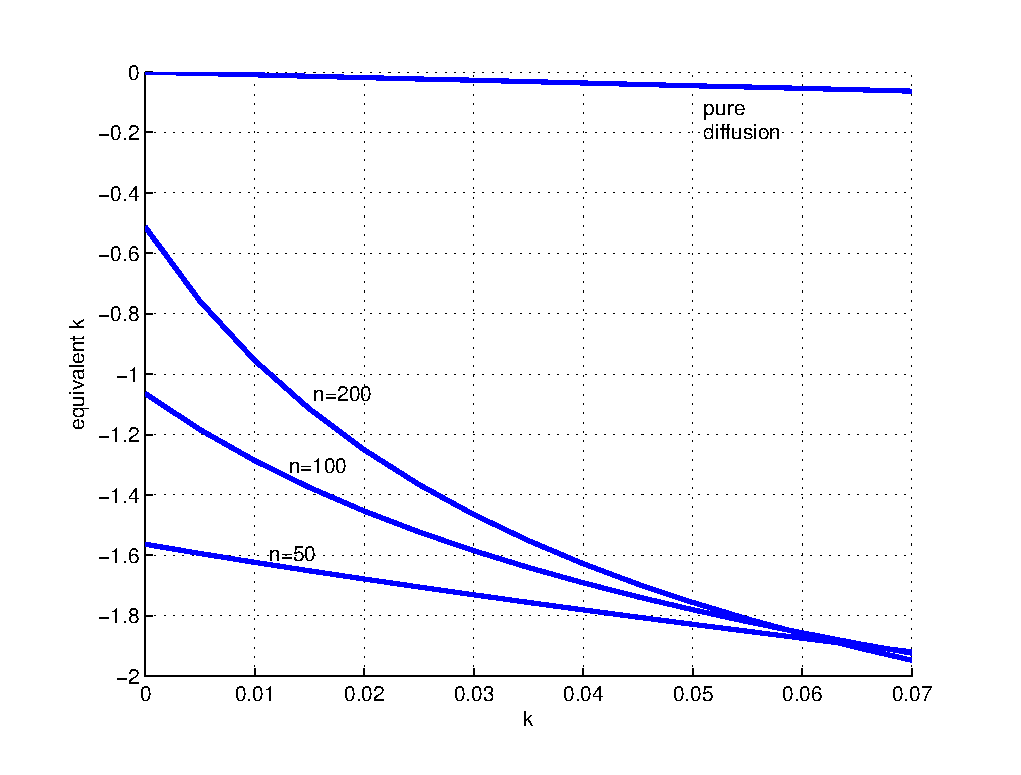
\includegraphics{standardmap_epsilon_0.2_kcompare.eps}}}


Normalize...

\centerline{\scalebox{0.5}[0.5]{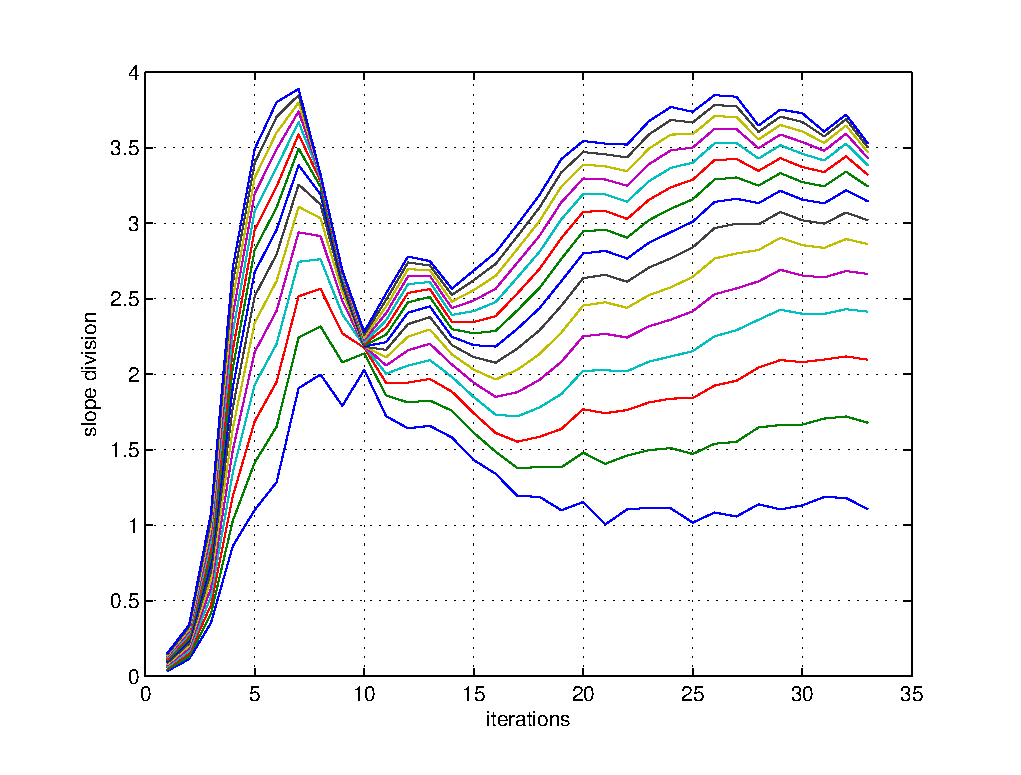
\includegraphics{standardmap_epsilon_0.2_slope_division.eps}}}


Now we compare different initial conditions
The four cases are: cos in x, cos in y, square wave in x, square wave in y

\centerline{\scalebox{0.5}[0.5]{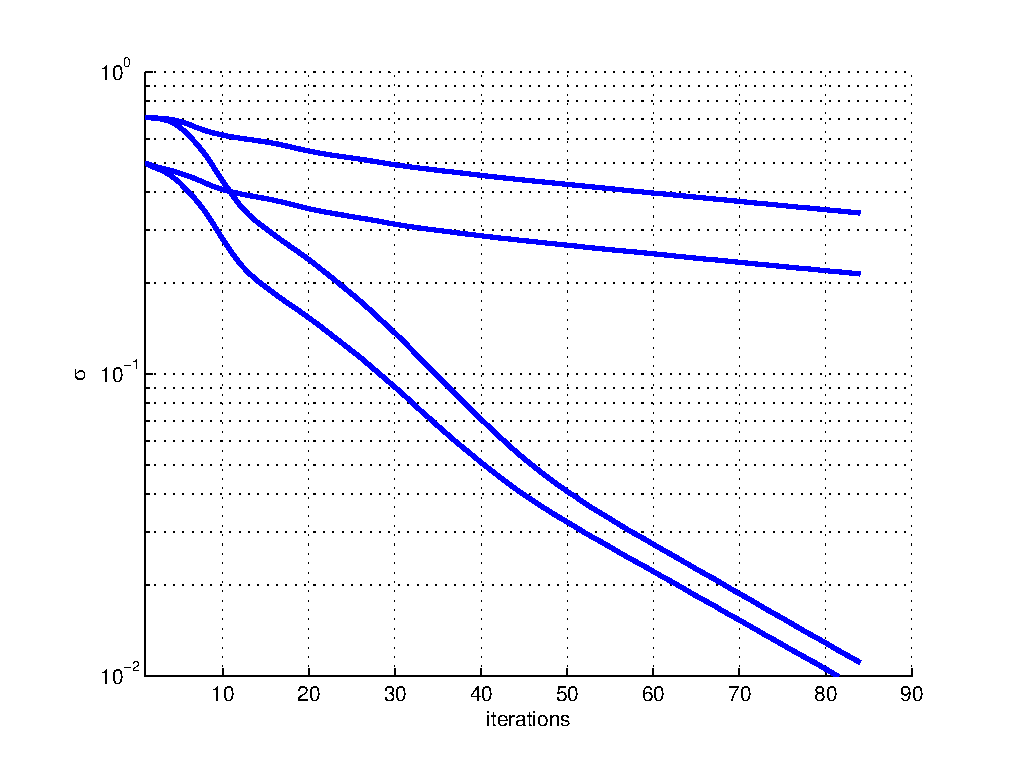
\includegraphics{compareinitial.eps}}}

Also, check the loglog plot. The initial condition is not on the
eigenfunction direction, so one shouldn't expect to see a straight line
in the first few iterations. This example is merely to show that $k$
has no effect to the doubly exponential term.

We assume in the first few iterations, $\sigma$ looks like
\begin{eqnarray}
 a e^{-b(2^{ct}-1)}
\end{eqnarray}
To get a slope $c$ curve, it is not just taking log twice!


\centerline{\scalebox{0.5}[0.5]{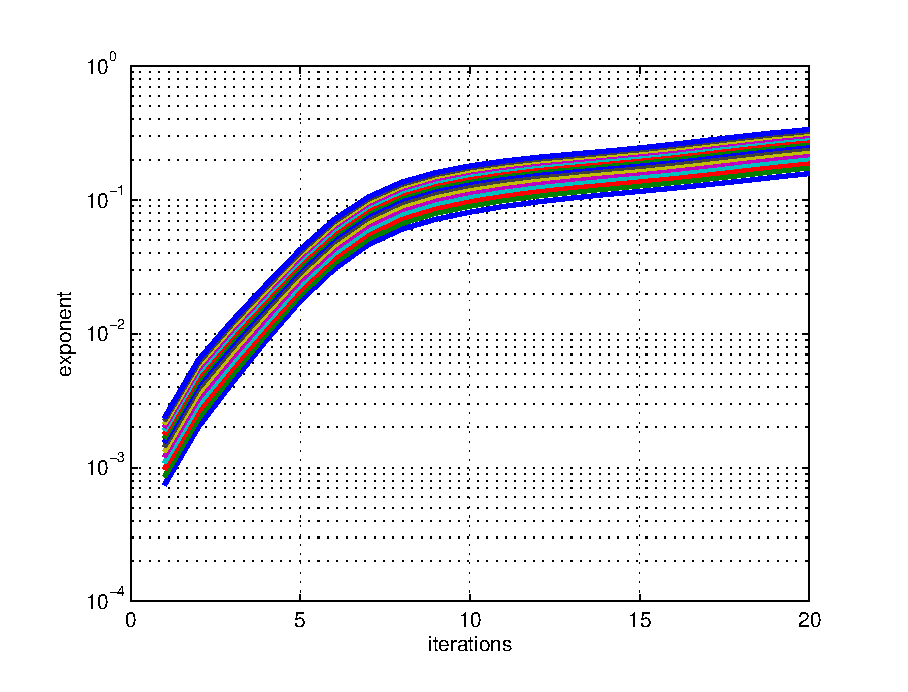
\includegraphics{loglog.eps}}}

%%%%%%%%%%%%%%%%%%%%%%%%%%%%%%%%%%%%%%%%%%%%%%%%%%%%%%%%%%%%%%%%%%%%%%%%%%%%%%%%%%%%

%%%%%%%%%%%%%%%%%%%%
\section{An Example}
%%%%%%%%%%%%%%%%%%%%
We will begin our discussion with an example simulated numerically,
it shows that the typical mixing enhancement by the map with
diffusion has two stages. The detail of how we simulate the system
will be given later. For now we just focus on the phenomenon.

\begin{example}

Consider the Standard map,
\begin{eqnarray}
\label{standard map}
S(x,y) =      \left[ \begin{array}{c}
                   x'\\
                   y'
                      \end{array} \right]=
              \left[ \begin{array}{cc}
                   x+y+\epsilon \sin{2 \pi x}  \\
                   y+\epsilon \sin{2 \pi x}
                      \end{array} \right]  (\mbox{ mod } 1)
\end{eqnarray}

where $\epsilon = 0.1$. The map with diffusibility $k = 1e-3$ and
$\Delta t = 1e-1 $ is simulated with initial density function
$c(x,y)$,
\begin{eqnarray}
c(x,y) = \left\{ \begin{array}{c}
          1  \mbox{  , if } 0\le x < \frac{1}{2}\\
          0  \mbox{  , if } \frac{1}{2} \le x < 1
          \end{array} \right.
\end{eqnarray}

After each iteration $\sigma$ is calculated. The $log$ plot of
$\sigma$ versus time is shown in figure \ref{example1} on a red
line. Without the map, the diffusion equation is solved analytically
and its $\sigma$ is plotted in the same figure with a blue line as a
comparison.

Since the $[M(k,t)]$ operator is symmetric and real, it has an
orthogonal eigenfunction structure. Each of the eigenfunction decays
independently in the rate proportional to its frequency. Hence the
blue curve asymptotes to the eigenfunction corresponding to the
second-largest eigenvalue.

On the other hand, the red line looks quite different. It drops
rapidly in the beginning and shows a concave shape. After a while
(in this examples, number of iteration larger than $10$), it
converges to a straight line which is the eigenfunction direction of
the map with diffusion operator.

\centerline{\scalebox{0.5}[0.5]{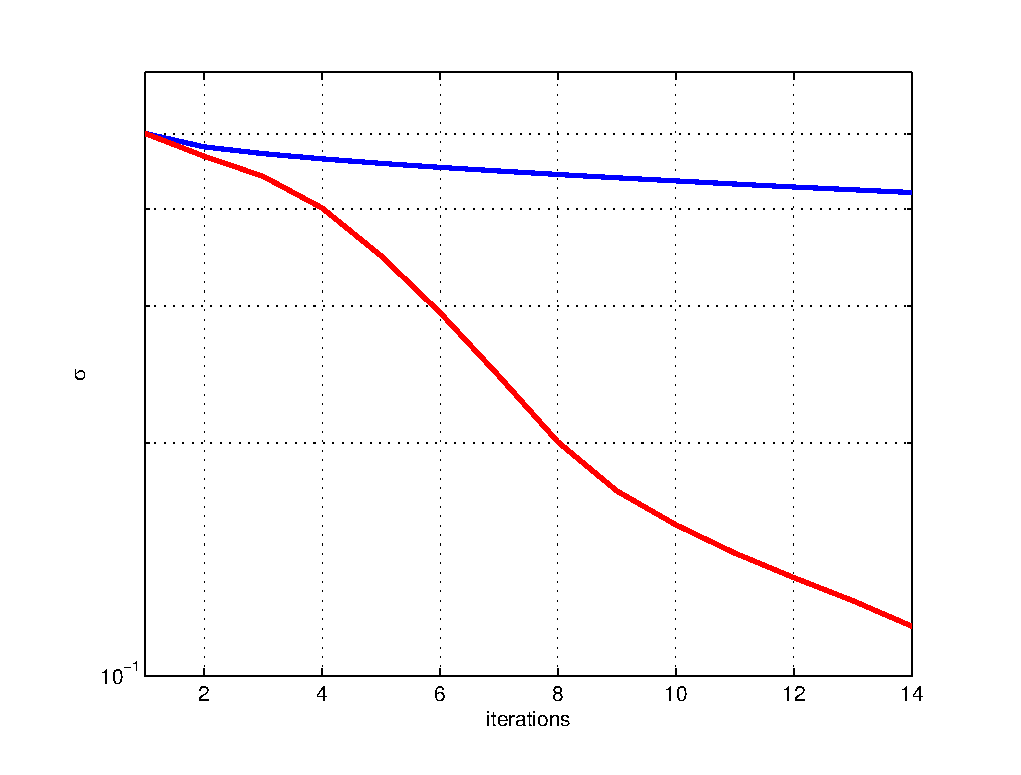
\includegraphics{example1.eps} \label{example1}}}

\end{example}

The map enhances the mixing in two ways,
\begin{enumerate}
 \item transiently, the map changes the convex curve to a concave one, this dramatically reduces $\sigma$ in the first few iterations.
 \item after a while, both red and blue lines tend to be straight with different slope. The red line is steeper, which means the map enhances the long-time mixing rate by a constant factor.
\end{enumerate}

The observation above suggests that to understand the enhancement
factor a map produces, one need to consider both the transient and
long-time enhancements.

%%%%%%%%%%%%%%%%%%%%%%%%%%%%%%%%%%%%%%%%%%%%%%%%%%%%%%%%%%%%%%%%%%%%%%%%%%%%%%%%%%%%%%%%%%%%%%


%%%%%%%%%%%%%%%%%%%%%%%%%%%%%%%%%%
\section{The Cutoff Phenomenon}
%%%%%%%%%%%%%%%%%%%%%%%%%%%%%%%%%%
We first consider an analytical solvable problem.
\begin{example}

The domain is still a 2-dimensional torus initially, but now the
continuous-time map stretches the coordinate as,
  \begin{eqnarray*}
     (x,y) \leftarrow (2^{-t}x_0,2^{t}y_0)\\
  \end{eqnarray*}
We assume the initial density function $c(x,y) = \bar{c}(x)$ is a
function of $x$ only, and thus it can be reduced to a 1-D problem.
One can work out that the diffusion equation with this coordinate
transformation is the PDE
  \begin{eqnarray*}
     u_t - u_y\log{2}  = k u_{yy}
  \end{eqnarray*}
The $u_y\log{2}$ term can be viewed as the diffusibility induced by
the coordinate transformation. Now let $v(y',t) = u(y,t)$, where $y'
= 2^{-t}y$ and also, implicitly $x' = 2^{t}x $, the PDE becomes
  \begin{eqnarray}
  \label{bakers pde on y'}
     v_t  = k 2^{2t} v_{y'y'}
  \end{eqnarray}
This coordinate transformation brings the domain back to a fixed 2-D
torus, on which we know how to solve the PDE. It is easy to show
that $[\sigma]u = [\sigma]v $. Let $\bar{c}(y) = \sum_{n=0}^\infty
cos(2 \pi n y) $, i.e., the Fourier series of $\bar{c}(y)$. The
solution of (\ref{bakers pde on y'}) is,
  \begin{eqnarray*}
     v(y',t) =  \sum_{n=0}^\infty c_n \cos (2 n \pi  y') e^{-\frac{4 k n^2 \pi^2 (2^{2 t}-1)}{2\log (2)}}
  \end{eqnarray*}
Calculate $[\sigma]u$ as
\begin{eqnarray*}
 [\sigma]u(x,y,t) = \left(\int_{0}^{1} v(y',t)^2 dx'\right)^{\frac{1}{2}} = \sum_{n=0}^\infty c_n 2^{-\frac{1}{2}} e^{-\frac{4 n^2 \pi^2 k (2^{2t}-1)}{2\log2} }
\end{eqnarray*}
So each of the term inside the summation decays doubly exponentially.

\end{example}

Consider the baker's map,
  \begin{eqnarray}
    S(x,y) =  \left\{ \begin{array}{cc}
                 (2x,\frac{1}{2}y) \mbox{ mod } 1      &\mbox{, if } 0\le x < \frac{1}{2} \\
                 (2x,\frac{1}{2}(y+1)) \mbox{ mod } 1  &\mbox{, if } \frac{1}{2}\le x< 1\\
              \end{array} \right.
  \end{eqnarray}
The above example is a continuous-time version of the baker's map with some specific initial condition. It explains why the baker's map mixes a density function doubly exponentially. In fact, this has been observed in many Markov chain simulation and is called cutoff phenomenon.


%%%%%%%%%%%%%%%%%%%%%%%%%%%%%%%%%%%%%%%%%%%%%%%%%%%%%%%%%%%%%%%%%%%%%%%%%%%%%%%%%%%%%%%%5
%%%%%%%%%%%%%%%%%%%%%%%%%%%%%%%%%%%%%%%%%%%%%%%%%%%%%%%%%%%%%%%%%%%%%%%%%%%%%%%%%%%%%%%%


%%%%%%%%%%%%%%%%%%%%%%%%%%%%%%%%%%
\subsection{Estimation of $D^*$}
%%%%%%%%%%%%%%%%%%%%%%%%%%%%%%%%%%
As we have stated above, the operator $P_h$ is an approximation of
$[P(D^*,1)]$. Now let us assume one can equate the following
\begin{eqnarray}
\label{PnandP}
 P_h[d_h] = [d_h][M(D^*,1)][P]
\end{eqnarray}
and the diffusion caused by $[d_h]$ is small enough comparing with
$D^*$. we now discuss how to estimate $D^*$ when a $P_h$ is given.
Moreover, we also show that $D^*$ is roughly independent of what
function $P_h$ operates on.


To do this, we can create a test function $\phi(\mathbf{x})$ such
that $[P]\phi(\mathbf{x})$ is known analytically, and then apply it
to the the both sides of (\ref{PnandP}). We get
\begin{eqnarray}
\label{PnandPphi}
 P_h[d_h]\phi(\mathbf{x}) = [d_h][M(D^*,1)][P]\phi(\mathbf{x})
\end{eqnarray}
Left hand side of (\ref{PnandPphi}) can be evaluated numerically and
right hand side of it is done analytically and written as a function
of $D^*$. Thus we can solve for $D^*_\phi$ for this specific
$\phi(\mathbf{x})$.

The set of test functions we choose are $\phi_{k_1,k_2}$ for
$k_1,k_2\in \mathbb{Z}^+$ such that $\phi_{k_1,k_2}(\mathbf{x}) =
\sin(2\pi k_1 x^s)\sin(2 \pi k_2 y^s)$, where $[x^s , y^s]=S(x,y)$.
This particular choice satisfies $[P]\phi_{k_1,k_2}(\mathbf{x})=
\phi_{k_1,k_2}(S^{-1}(\mathbf{x})) = \sin(2\pi k_1 x)\sin(2 \pi k_2
y)$ and thus
\begin{eqnarray}
\label{MPphi}
 [M(D^*,1)][P]\phi_{k_1,k_2}(\mathbf{x}) = \sin(2\pi k_1 x)\sin(2 \pi k_2
y)\text{e}^{-4 \pi^2 (k_1^2+k_2^2)D^*}
\end{eqnarray}
Substitute the above equation to (\ref{PnandPphi}) and calculate the
2-norm of both sides, one can easily get the average of
$D^*_{\phi_{k_1,k_2}}$ over the domain $T^2$. The result of
estimated $D^*_{\phi_{k_1,k_2}}$ for $k_1=k_2 = k$ is plotted in
figure \ref{estimateddiffusionrate}.

Because in the process of approximating the map by a Markov matrix,
the diffusion is not added uniformly, one should not get a perfectly
consistent $D^*$ for every function and for the whole domain.
However, in figure \ref{estimateddiffusionrate} one can clearly see
when $n$ is large enough, $D^*_{\phi_{k_1,k_2}}$ is close to a
constant for different wave numbers $k$. The reason that all the
curves drop when $k$ gets higher is because the $[d_h]$ operator
itself is diffusive and this effect is not ignorable when $k$ is
large. One should not expect $n=50$ to capture any correct
information with wave number higher than $25$!

This figure gives us the idea of how large the augmentative
diffusivity rate is when $P_h$ is used to replaced $[P]$ and only a
range of wave number is considered.

We choose $D^* = D^*_{\phi_{1/10h,1/10h}}$ as the nominal diffusion
rate for $P_h$. It is not surprising that $D^*_{\phi_{1/10h,1/10h}}$
is linear to $\frac{1}{1/h^2}$. In figure \ref{ndchart} $P_h$ of
several different maps are calculated, and the
$D^*_{\phi_{1/10h,1/10h}}$ is then estimated by the above method.
Clearly one has
\begin{eqnarray}
\label{MPphi} D^*_{\phi_{1/10h,1/10h}} = c_s h^2
\end{eqnarray}
for some constant $c_s$, which is different from map to map.




%\begin{figure}
%\caption{\label{estimateddiffusionrate} The estimation of $D^*$ for
%different number of grids, as a function of wave number}
%\centerline{\scalebox{0.5}[0.5]{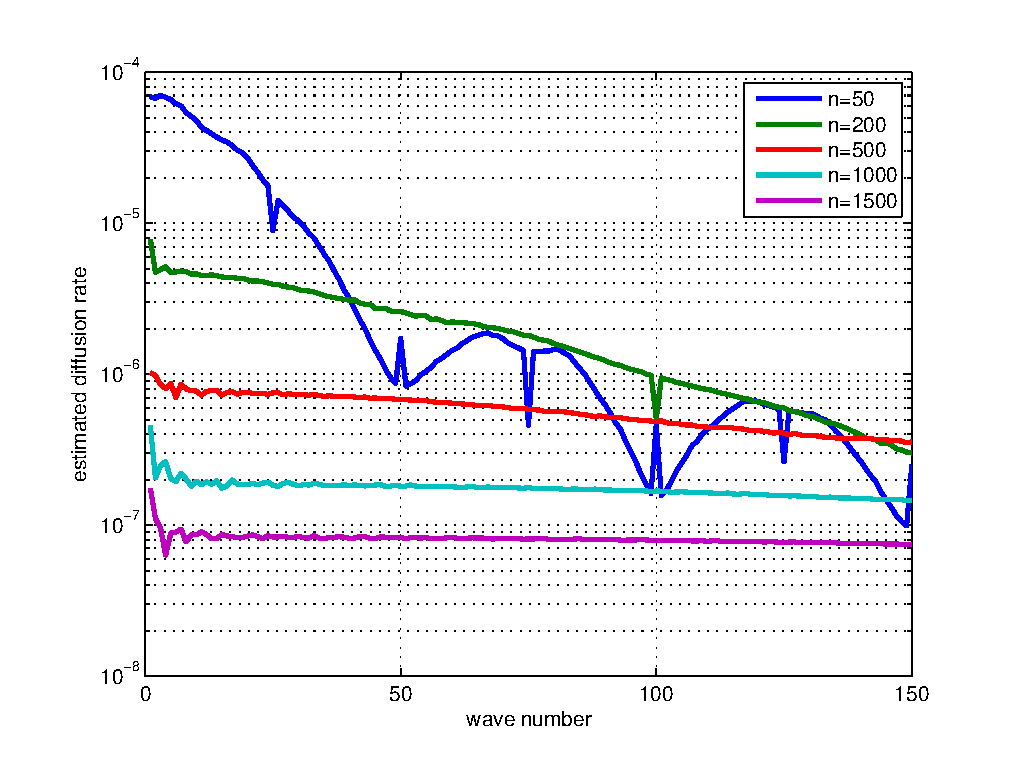
\includegraphics{estimateddiffusionrate.eps}}}
%\end{figure}
%\begin{figure}
%\caption{\label{ndchart} $D^*$ as a function of $\frac{1}{n^2}$, for
%different maps }
%\centerline{\scalebox{0.5}[0.5]{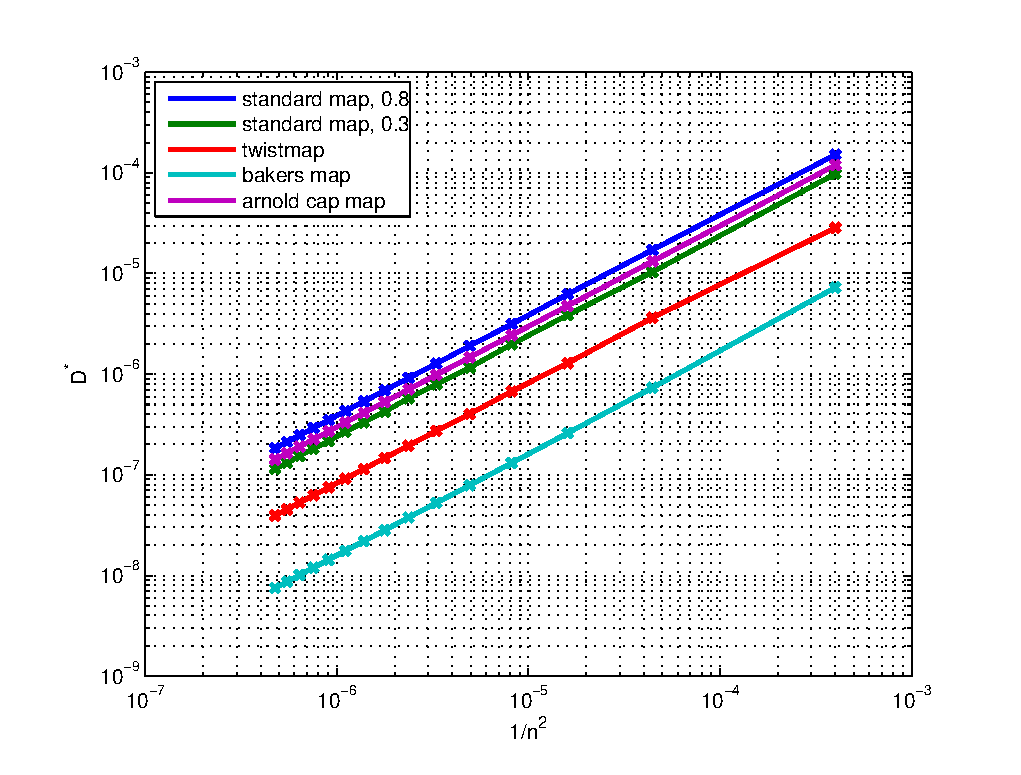
\includegraphics{ndchart.eps}}}
%\end{figure}


\begin{figure}
\centerline{\scalebox{0.5}[0.5]{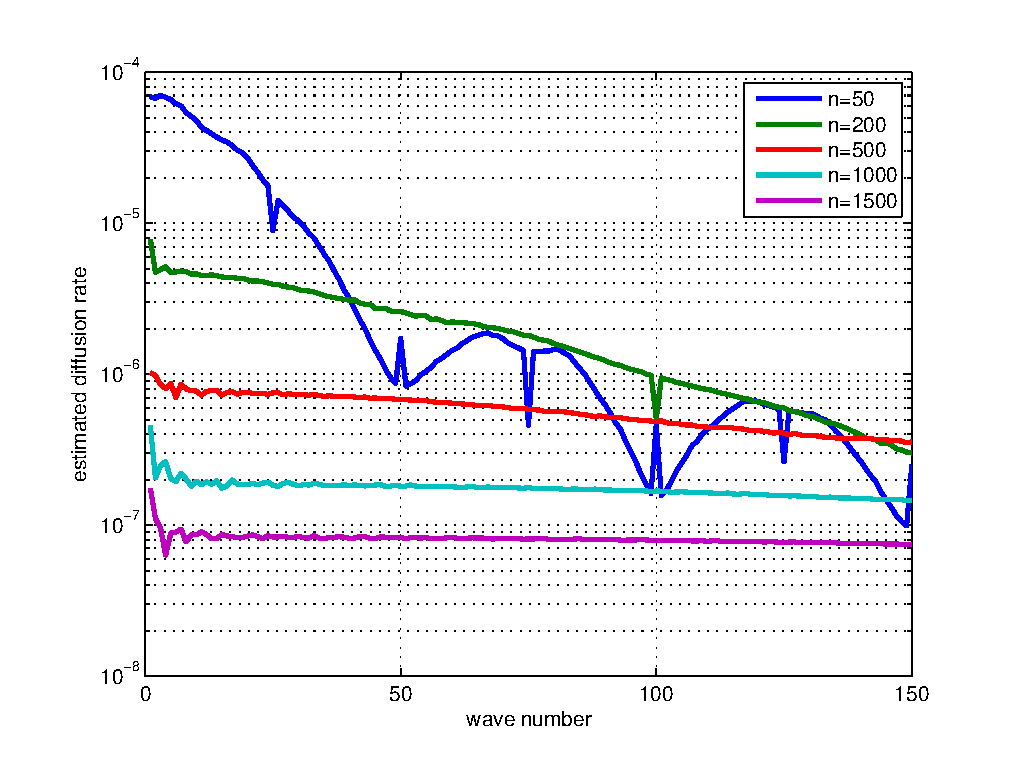
\includegraphics{estimateddiffusionrate.eps}}
            \scalebox{0.5}[0.5]{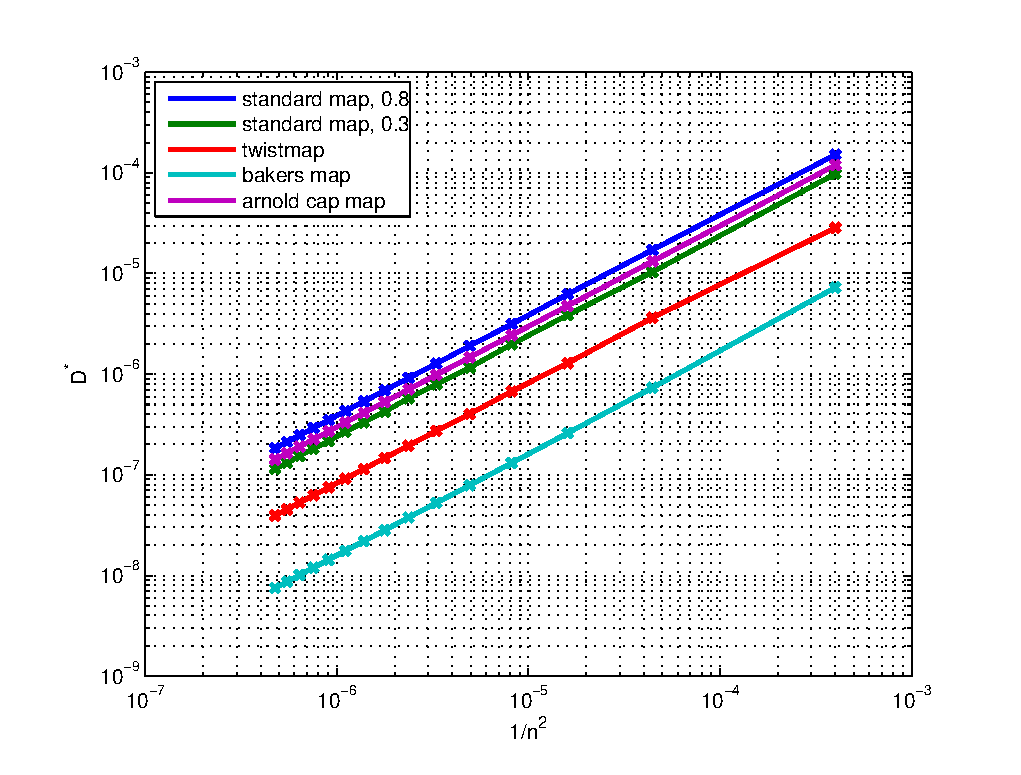
\includegraphics{ndchart.eps}}}
\caption{\label{ndchart} $D^*$ as a function of $h^2$, for
different maps } \caption{\label{estimateddiffusionrate} The
estimation of $D^*$ for different number of grids, as a function of
wave number}
\end{figure}

\subsection{Optimization of Mixing Protocol}
The goal of this $P_h$ operator is to deal with the design problem of microfluidic channels.
More speficifically, we formulate a periodical microfluidic channel as a map-with-diffusion
operator, and thus it can be optimized when certain objective function is given. The detail
of the formulation will be discussed later. Here we would like to address the scale issues.

As we have disscussed in the previous section, the diffusivity rate $D^*$ of $P_h$ is
proportional to $h^2$. Practically, one can add more diffusion without any difficulty,
but the only way to reduce the diffusion is to use a larger $1/h$. Here we would like to give a
rough estimation of the number on $1/h$ one needs when physical parameters are considered.

We adopt the parameters used in \ref{stroock2002}. Consider mixing a stream of protein
solution in aqueous buffer: molecular weight $10^5$, molecular diffucivity
$D_m~10^{-6} \text{cm}^2/\text{s}$. The mixing channel has cross sectional dimension
$200\mu \text{m}$ and length around $3\text{cm}$. Converting this set of parameters to a unit
square where $P_h$ operater is calculated from, one can deduce the diffucivity rate needed is
around $D =5 \times 10^{-5}$. According to figure \ref{estimateddiffusionrate}, $1/h=500$ is quite
sufficient for every map.


%%%%%%%%%%%%%%%%%%%%%%%%%%%%%%%%%%%%%%%%%%%%%%%%%%%%%%%%%%%%%%%%%%%%%%%%%%%%%%%%%5
%%%%%%%%%%%%%%%%%%%%%%%%%%%%%%%%%%%%%%%%%%%%%%%%%%%%%%%%%%%%%%%%%%%%%%%%%%%%%%%%%%

%%%%%%%%%%%%%%%%%%%%%%%%%%%%%%%%%%
\section{A Frequency Domain Approach}
\label{A Frequency Domain Approach}
%%%%%%%%%%%%%%%%%%%%%%%%%%%%%%%%%%

We would like to also discuss a model of the map with diffusion in
frequency domain. The goal of this model is not to simulate the map
with diffusion in a simpler way or to provide us an objective
function to optimize. Instead, we use the frequency domain model to
study how diffusion enhances the mixing.


\subsection{The Model and the Simplifications}

 We Fourier expand $w_n$ in
2-d,
\begin{eqnarray}
(w_h)_{p,q} =\sum_{s=0}^{1/h-1} \sum_{r=0}^{1/h-1} (\hat{w}_h)_{r,s}
e^{2 \pi j p rh} e^{2 \pi j q sh}  \mbox{   for }p,q \in
\{0,1,...,1/h-1\}
\end{eqnarray}
where $j = \sqrt{-1}$. The inverse discrete Fourier transform is
linear so we can rewrite the above equation as,
\begin{eqnarray}
w_h = F^{-1} \hat{w}_h
\end{eqnarray}
where $F^{-1} \in \mathbb{C}^{1/h^2 \times 1/h^2}$, $F^{-1}_{rs,pq}
=e^{2 \pi j h ({pr}+{qs}) i}$ for $p,q,r,s = 0,...,1/h-1$. Similarly the
forward transform can be denoted as $F$. Substitute the transforms
into the relation $w_h^{l+1} = P_h w_h^l$, one gets
\begin{eqnarray}
\hat{w}_h^{l+1} &=&F P_h F^{-1} \hat{w}_h^l \nonumber\\
          &\equiv& \hat{P}_h \hat{w}_h^l
\end{eqnarray}
Even though we have a really sparse $P_h$, the two dense matrices
$F$ and $F^{-1}$ spoil all the sparsity. Hence it is not wise to
evolve the system in frequency domain. However, just like in the
space domain, most of the entries in $\hat{P}_h$ could be very small.
Making those small entries zero, one can perhaps result in a sparse
operator in the frequency domain again. Nonetheless, the computation
cost is already huge when deciding which entry can be ignored, and
the operator one gets is far less sparser than $P_h$ in general.

Therefore, a further simplification is required to make the problem
more achievable. Let us start from observing what the most important
components are in frequency domain when a system evolves. Selecting
these components out of the others is our basic strategy to reduce
the size of of the model.


Suppose we only focus on a certain set of initial conditions, for
example, if one chooses $w_h^0 = [d_h][\cos(x)]$, then $\hat{w}_h^0$
has only a single nonzero component. As the system evolves,
$\hat{w}_h^l$ gets more and more non-zeros. Meanwhile, each of the
components also decays in various rates. And finally, when the two
effects balance, the system arrives at its eigenfunction direction,
which only has a limited number of nonzero frequencies. In this
whole procedure, three simplifications can be done:
\begin{itemize}
  \item We restrict the initial condition to be some simple
  functions, which do not have too many components in the frequency
  domain.
  \item When the system evolves, we keep recording the states it
  passes through. We set a threshold, and only the states whose
  absolute values are higher than the threshold are kept. Thus we can get how
  many significant $m$ states we needs to simulate the system.
  \item The reduced operator, called $\hat{P}_m \in \mathbb{C}^{m \times m}$,
  is formed by selecting the corresponding entries in $\hat{P}$. When
  doing this, we also set the entries whose absolute values are
  below the threshold to be zero.
\end{itemize}

It seems very restrictive when we say the initial condition is a
"simple function". Nonetheless, considering that we are studying the
mixing property of a map, to begin with a simple function which has
only few nonzeros in frequency domain is actually reasonable.
Moreover, on the 2-d domain with $1/h$ by $1/h$ grids, even for a step
function in $x$-direction has only $1/h$ nonzero components-still
pretty sparse.

The second simplification is the key to decide the size of the
reduced system. One can certainly image how the number of nonzero
states grows when the system evolves-it grows exponentially.
However, most of the components are mapped from low frequency states
to high frequency ones. This means a large amount of them decays
fast and becomes insignificant before the system arrived at its
stationary state. Deleting these states from our simulation should
not affect too much. Besides, one can always adjust the threshold
value to move between a more accurate model and a compact one.

The above step is equivalent to
\begin{eqnarray}
\label{Prmodel}
    \hat{P}_m(D^*) = F_m P_n(D^*) F_m^T
\end{eqnarray}
where $F_m$ is composed by the selected rows of $F$, and because $F$ is unitary, $F^{-1} = F^T$,
$F_m^T$ is the selected columns of $F^{-1}$. If the number of selected states is much smaller than
$1/h^2$, the $\hat{P}_m$ model can be evolved efficiently.

Suppose the selected $m$ states have indice $(r_i,s_i)$, for $i=1,...,m$
in the 2-d representation of $\hat{w}_h$, and each of them has the
corresponding wave number $\mathbf{k}_i = \sqrt{(k_1)_{r_i}^2+(k_2)_{s_i}^2}$.
Let $\hat{k}_m = [\mathbf{k}_1, \mathbf{k}_2,...,\mathbf{k}_m ]$.
If one want to study how the system behavior changes when more diffusion is added.
It is equivalent to pre- or post-multiply the $\hat{P}_r$ model by a diagonal matrix,
\begin{eqnarray}
\label{PraddDiffusion}
    \hat{P}_m(D) = \hat{P}_m(D^*)\text{e}^{-4 \pi^2 (D-D^*) \text{diag}(\hat{k}_m^2)}
\end{eqnarray}

If the above simplifications have resulted in a moderate size system,
the thrid part is not necessary. However, setting the small nonzeros
zero helps us to identify the most important paths which connect the
initial condition to the stationary state.



\subsection{Simulations}
We set the threshold value in the second and the third steps of simplifications
 to be $0.01$. In figure \ref{PrchangeD} we compare the $P_h$ model and the $\hat{P}_m$ model for
standard map with $\epsilon=0.2$ and initial condition $\cos(x)$. In the $P_h$ model, we use fixed number of grid $1/h = 200$.
The corresponding $D^*$ is $4.21e-6$ and number of states is $1/h^2 = 40000$. The solid lines show the $P_h$ model with some augment diffusion added by using
Discrete Fourier transform technique on $w_h^l$ after every iteration. $\hat{P}_m$ model is calculated by
equation (\ref{Prmodel}) using the raw $P_h(D^*)$ model. The $\hat{P}_m$ model has only $4326$ states. Its diffusion is added by applying equation (\ref{PraddDiffusion}) and plotted in dased lines.

The main advantage of the $\hat{P}_m$ model is of course not in the simulation. It provides us an efficient way to study how the diffusion affects the system behavior. Suppose we focus on the exponentional region of the convergence curve, figure (\ref{Dvslambda}) shows how the diffusion affects the decay rate when the system is in its eigenvector direction. The map is standard map with various chaotic parameters $\epsilon$. Although the theorem about the eigenvalue perturbation when a diagonal matrix is multiplied is not known. The numerical simulations do show a roughly linear relation when $\epsilon$ is small.




\begin{figure}
 \centerline{
  \scalebox{0.5}[0.5]{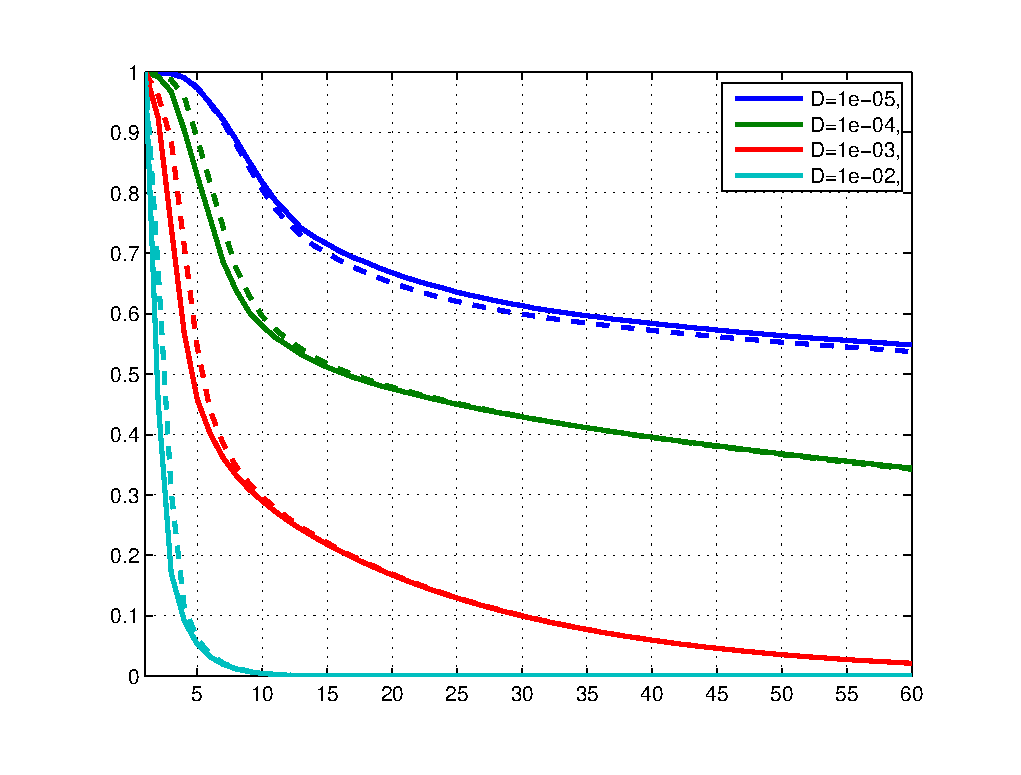
\includegraphics{PrchangeD.eps}}
  \scalebox{0.5}[0.5]{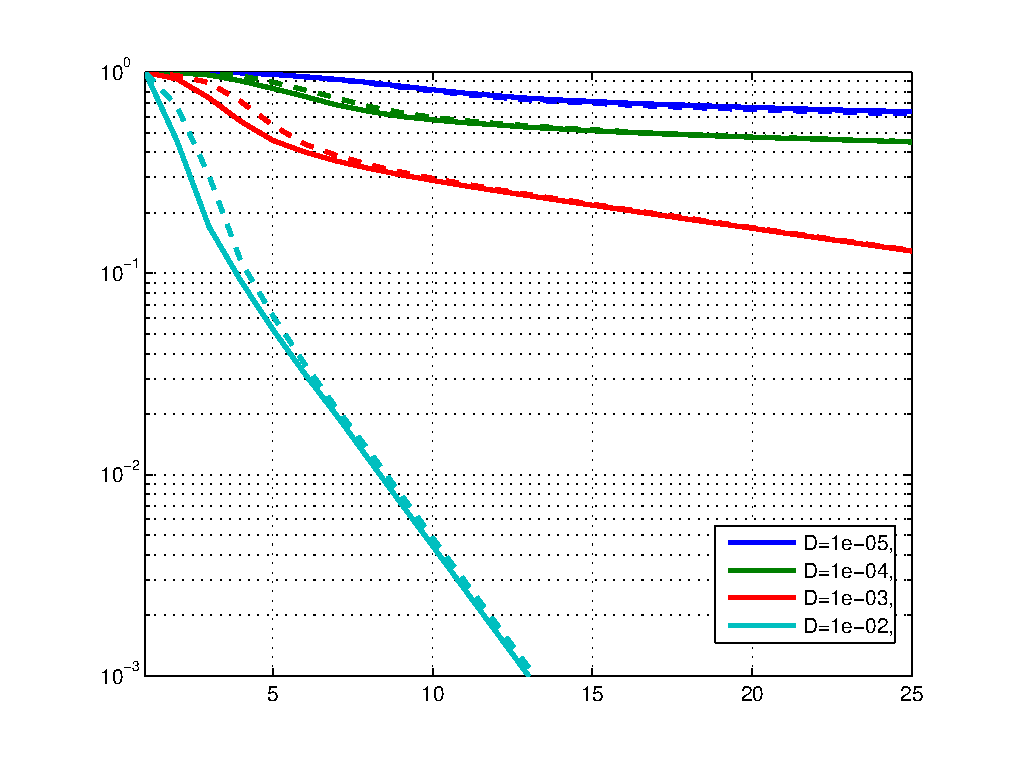
\includegraphics{PrchangeDlog.eps}}
} \caption{ddd}
  \label{PrchangeD}
\end{figure}


\begin{figure}
 \centerline{
  \scalebox{0.5}[0.5]{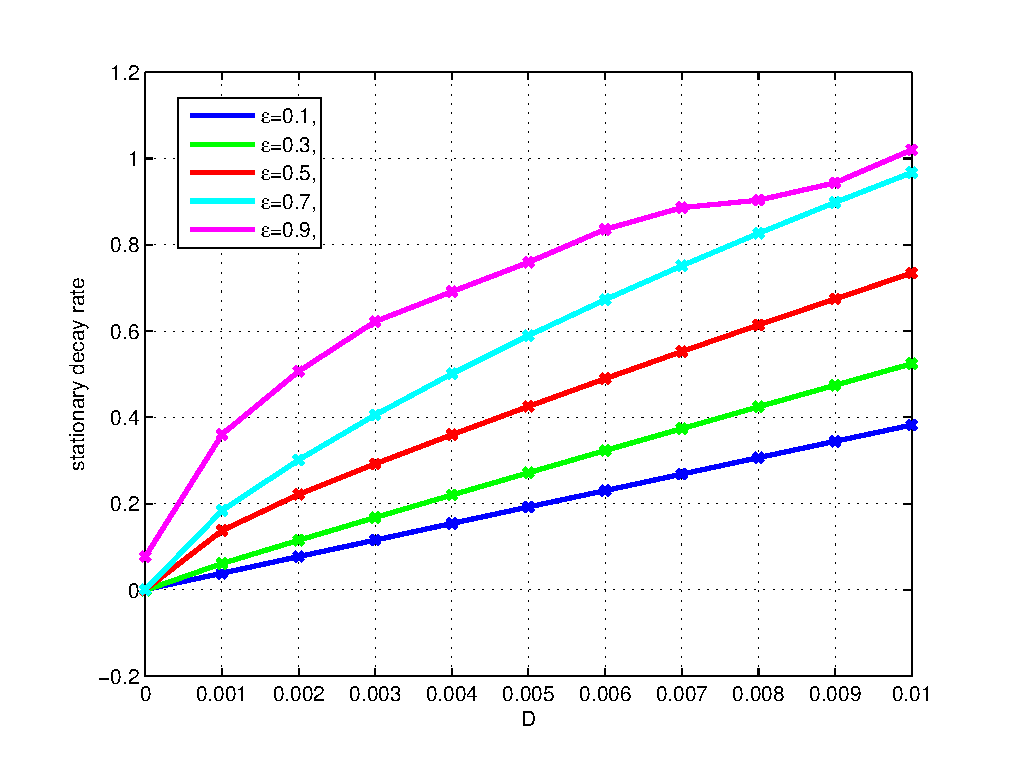
\includegraphics{Dvslambda.eps}}
} \caption{ddd}
  \label{Dvslambda}
\end{figure}


\subsection{Mixing Enhancement Factor}

%%%%%%%%%%%%%%%%%%%%%%%%%%%%%%%%%%%%%%%%%%%%%%%%%%%%%%%%%%%%%%%%%%%%%%%%%5
%%%%%%%%%%%%%%%%%%%%%%%%%%%%%%%%%%%%%%%%%%%%%%%%%%%%%%%%%%%%%%%%%%%%%%%%%%
%\subsection{An Approximation of $P_h$}
%
%In reality, to calculate each nonzero $(P_h)_{ij}$ using (\ref{P definition}), one needs to integrate $\pi$ over the intersection of two polygons. The number of nonzero is about order $4/h^2$ to $8/h^2$. For a large $1/h$, the computation% cost is huge. To overcome this, we suggest a series of simplification.

%Let $I = \{(i,j)|(P_h)_{ij} \neq 0\}$ be the set of nonzero index of $P_h$. The nonzero pattern is assumed known and accurate. Given a very rough estimation of $P_h$, called $\tilde{P}_h$, which has the same nonzero pattern as $P_h$ but each of the nonzero entry is just an estimation of $(P_h)_{ij}$. Solve the following linear program,
% \begin{eqnarray}
% \label{LPforP}
%       min  & \sum_{(i,j)\in I} |(\tilde{P}_h)_{ij} - (\bar{P}_h)_{ij}|\\
%       s.t. & \bar{\pi}_h^T \bar{P}_h = \bar{\pi}^T   \nonumber\\
%            & \bar{P}_h \mathbf{1}  = \mathbf{1}   \nonumber\\
%            & (\bar{P}_h)_{ij} \ge 0    \mbox{  , for all }(i,j) \in I \nonumber
% \end{eqnarray}
%The linear program has number of variables and inequality constraints equal to the number of members of $I$, and $2/h^2$
%equality constraints. In general it is tight enough to get a good approximation of $P_h$ because the nonzero pattern and the
%row/column sums are much more important than the exact number of each $(P_h)_{ij}$.

%As for $\tilde{P}_h$, some very cheap estimation can be applied, here is the one we suggest. Suppose $(\tilde{P}_h)_{ij}$ is known to be nonzero. The $i-$ and $j-th$ cells center at $(i_x,i_y)$ and $(j_x,j_y)$, respectively. Let $(j_x^{S^{-1}},j_y^{S^{-1}}) = S^{-1}(j_x,j_y)$, then
%\begin{eqnarray}
% \label{arearaitioeq}
% (\tilde{P}_h)_{ij} = |(|i_x-j_x^{S^{-1}}|)-l_x| \cdot |(|i_y-j_y^{S^{-1}}|)-l_y|
%\end{eqnarray}
%where $l_x$ and $l_y$ are the lengths of each cell in $x$ and $y$ directions. This is of course a very rough estimation of$S^{-1}(a_j) \cap a_i$, but it turns out to be good enough. One should be notified that this estimation is only valid when${P}_{ij}$ is actually a nonzero. If one misuses this estimation on a zero entry, the result would be completely wrong. Conversely, if for some of the entries which are nonzero but we set them to be zero, the global effect is extremely small.


%\subsection{A Further Approximation}
%
%The above strategy can easily convert a map $S$  to a Markov matrix $\bar{P_h}$ if one chooses the grid in each direction to be around several hundreds. However, because the linear program (\ref{LPforP}) has number of variables $O(1/h^2)$, for large $1/h$ the computation cost is still high. Thus for the size of $P_h$ larger than 500, we recommend to use $\hat{P_h}$ as a substitution of $\bar{P_h}$, $\hat{P_h}$ is
% \begin{eqnarray}
%    (\hat{P_h})_{ij}  = \frac{(\tilde{P_h})_{ij}}{\sum_j (\tilde{P_h})_{ij} }
% \end{eqnarray}
%which is just $\tilde{P_h}_{ij}$ normalized by each row. $\hat{P_h}$ clearly satisfies  $\hat{P_h} \mathbf{1}  = \mathbf{1}$, but not $\pi_h^T \hat{P} = \pi_h^T$ in general. However, one can find its invariant distribution $\hat{\pi_h}$ by simulation. In all our experiments with $1/h \geq 200$, $\hat{\pi_h}$ is almost the same as $\pi_h$, which means $\hat{P_h}$ is indeed a good approximation for $P_h$. In fact, because it is extremely efficient to compute $\hat{P_h}$ even for $h$ up to one or two thousands, $\hat{P_h}$ is much more useful when one want to observe the details of how the function evolves. Hence we will use $\hat{P_h}$ as $P_h$ when $1/h \geq 200$ and $\bar{P_h}$ when $1/h < 200$, in the rest of this paper.


%%%%%%%%%%%%%%%%%%%%%%%%%%%%%%%%%%
\subsection{About the Error}
%%%%%%%%%%%%%%%%%%%%%%%%%%%%%%%%%%
In this subsection we derive the error of the $P_h$ operator after
one iteration. This algorithm is first order accuracy to approximate
the Perron-Frobenious operator.


Let $\mathbf{x}_i = (x_i,y_i)$ be the center of cell $a_i$, and $f_i
= f(\mathbf{x}_i)$ denotes the function value at $\mathbf{x}_i$, and
$F_i$ is the function value calculated by our algorithm. Let
$\mathcal{J}_i = \{j | S^{-1}(a_i) \cap a_i \neq \emptyset\}$. Now
suppose at iteraiton $l-1$ the function $f_j^{l-1}$ is known exactly
for every $j \in \mathcal{J}$. Define the error of $P_h$ on cell $i$
at iteration $l$ to be $e_i^l$,
\begin{eqnarray}
e_i^l = F_i^l - f_i^l
\end{eqnarray}
where $F_i^l$ can be represented by the $P_h$ operator and $f_j^{l-1}$,
\begin{eqnarray}
F_i^l = \sum_{j \in \mathcal{J}_i} (P_h)_{ij} f_j^{l-1}
\end{eqnarray}
and now we Taylor expand $f_j^{l-1}$ about $f(S^{-1}(\mathbf{x}_i))$,
\begin{eqnarray}
f_j^{l-1}  = f^{l-1}(\mathbf{x}_i) +
\frac{\partial{f^{l-1}}}{\partial{\mathbf{x}_i}}
(\mathbf{x}_j-S^{-1}(\mathbf{x}_i))
           + \text{O}((\mathbf{x}_j-S^{-1}(\mathbf{x}_i)^2))
\end{eqnarray}
Substitute above relations into the error equation, one has
\begin{eqnarray}
e_i^l = \sum_{j \in\mathcal{J}_i} (P_h)_{ij}
\left(f^{l-1}(S^{-1}(\mathbf{x}_i))
        + \frac{\partial{f^{l-1}}}{\partial{x}} (\mathbf{x}_j-S^{-1}(\mathbf{x}_i))
        + \text{O}((\mathbf{x}_j-S^{-1}(\mathbf{x}_i)^2))\right) - f_i^l
\end{eqnarray}
Note that in any of our simplifications,
\begin{eqnarray}
f_i^l = \sum_{j \in \mathcal{J}_i} (P_h)_{ij}
f^{l-1}(S^{-1}(\mathbf{x}_i))
\end{eqnarray}
because $P_h$ is a stochastic matrix. Therefore one concludes

\begin{eqnarray}
e_i^l = \sum_{j \in \mathcal{J}} (P_h)_{ij} \left(
\frac{\partial{f^{l-1}}}{\partial{\mathbf{x}}}
(\mathbf{x}_j-S^{-1}(\mathbf{x}_i))) + \text{O}((\mathbf{x}_j-S^{-1}(\mathbf{x}_i)^2))\right)
\end{eqnarray}
$(P_h)_{ij}$ is the weighted area ratio. Clearly no matter it is
calculated by (\ref{arearaitioeq}) and then normalized or by (\ref{P
definition}) numerically, the error does not scale with $h$. The
$(\mathbf{x}_j-S^{-1}(\mathbf{x}_i))),{j \in \mathcal{J}_i}$ term is
the $x$ and $y$ distance of $S^{-1}(\mathbf{x}_i)$ to the grid
points, so it scales with $h$. Thus we can conclude this algorithm
has first order accuracy and when $h \rightarrow 0$, $F_i^l$
converges to $f_i^l$.

% scales with ???

One can view the above error $e_i^l$ as some artificial diffusion on
grid $i$. Because of this artificial diffusion, the operator $P_h$
is in fact more close to $[P(D^*,1)]$ rather than $[P]$. Although
$e_i^l$ is not uniform over the domain and scales different from the
physical diffusion $D^*$, we can still find an equivalent $D^*$ for
every $P_h$, and when

%%%%%%%%%%%%%%%%%%%%%%%%%%%%%%%%%%%%%%%%%%%%%%%%%%%%%%%%%%%%%%%%%%%%%%%%%%%%

\section{Some Facts}




\subsection{The Convexity of Eigenvalue Functions}
The maximum eigenvalue of a symmetric matrix, i.e., $\lambda_{1}(A)$ is convex.

The second largest eigenvalue of a doubly stochastic symmetric matrix is convex.

$$\lambda_{2}(P)=\sup\{u^{T}Pu \,|\, \|u\|_{2}\le1, \mathbf{1}^{T}u=0\}$$

The negative of the smallest eigenvalue is also convex,

$$-\lambda_{n}(P)=\sup\{ -u^{T}Pu \,|\, \|u\|_{2}\le1 \}$$

Hence, SLEM $\mu(P)=max\{\lambda_{2}(P),-\lambda_{n}(P)\}\,$is convex.


%%%%%%%%%%%%%%%%%%%%%%%%%%%%%%%%%%%%%%%%%%%%%%%%%%%%%%%%%%%%%%%%%%%%%%%%%%%%%%

\subsection{Cut-off phenomenon and mixing problem}
Now we try to make connections between the well-known cut-off phenomenon in simulating some Markov chains and the mixing process. A mixing model is introduced to explain the cut-off phenomenon. The model has two phases, and they are corresponding to the two stages we observe in before and after a cut-off, respectively. 

Cut-off phenomenon has been observed in many Markov chain simulations. The most famous example is the riffle-shuffle problem. It has been shown that the total variance distance between the current state and the stationary distribution exhibits a sharp drop at around the seventh shuffle. Before this point it tends to a one doubly exponentially decay, and past this point the distance tends to $0$ exponentially. 

There are several things need to be notified before our discussion. First, whether the cut-off happens depends on the initial state. One can always find an initial distribution which has no cut-off by simply choosing the left eigenvector (of the Markov matrix) direction. Secondly, there is no cut-off if the Markov matrix is symmetric. In this case, the left eigenvectors are orthogonal to each other so for any initial state it can be decomposed into a unique linear combination of these left eigenvectors, and hence each of the components decays exponentially. Thirdly, the term D-cut-off is used to indicate the cut-off with measure D. D can be the total variation distance, the separation or the 2-norm distance, etc. It is possible that the cut-off happens in one measure but not in another, or they cut at different positions. Finally, it is still not well understood how cut-off happens, and it seems like there are several different kinds of cut-offs that satisfies the defition. The model we use is not trying to explain ALL the cut-off phenomenon, but to describe one of the possible reason.    

We assume the mixing process is a markov process with uniformly stationary distribution. So we have
\begin{eqnarray*}
  x^{k+1} &=& A^{T}x^{k}\\
  \mathbf{1} &=& A^{T}\mathbf{1}
\end{eqnarray*}
In this case, when $x = \mathbf{1}$ a function is transported by the matrix $A$, 
\begin{eqnarray*}
  f^{k+1} &=& A^{T}f^{k}\\
\end{eqnarray*}
So when we talk about mixing of the Markov chain, we actually refer to the property that how the function tends to its average everywhere. Assume the following, 
 \begin{eqnarray*}
  A = MP
\end{eqnarray*}  
where $P$ is a permutation matrix and $M$ is a symmetric matrix. By this we mean the effect of $A$ acting on a function $f$ is first to diffuse the entries of $f$ by $M$ and then permute according to $P$. The way to decompose $A$ into $M$ and $P$ is unrelated to this disscusion. Here we simply want to point out that if the above condition holds, how the cut-off happens.   

We define the domain is a 2-d torus with $n$ grids at each side, and $n$ is large. As usual, we use the vector $f$ to represent the "color", $f \in [0 ,1]^{n^2} $. $f^0$ is totally unmixed so $f \in \{0 ,1\}^{n^2}$. Define the $l$ to be the boundry length (need a clear definition). 

Define $\sigma$ to be the 2-norm of the $f- f_{ave}$.    

\subsubsection{Phase One}
If we apply only $M$ to $f^0$, the thing we will observe is the on the boundry the "color" diffuses and smooth out $f$. It is clear that the $\sigma = c \cdot l^{-dk}$, where $c$ and $d$ are constants, and $k$ is the number of iterations . If we then apply $P$, in general we will see $l$ grows exponentially, so $l=l(t)= l_{0} \cdot e^{ak}$ for some constant $a$ and initial length $l_{0}$. Combine the two observations we get 
\begin{eqnarray*}
  \sigma = c \cdot (l_{0} \cdot e^{ak})^{-dk}
\end{eqnarray*}  
This explains why $\sigma$ drops one doubly exponentially in the begining. Of course the assumption of this to happen is that along the boundry there is a small diffusion region, the boundy should not twist too much so that these regions stack on each other.    

\subsubsection{Phase Two}
The above rapid drop lasts for a certain amount of iterations until the assumption doesn't hold anymore. Then we can assume that the distribution is now on the space spamed by $v_1$ and $v_2$. This is because $v_1$ is the dircetion that never diffuses (it is the uniformin distribution) and $v_2$ is the one that diffuses most slowly. Hence the distance now decays exponentionally with the rate $\lambda_2(MP)$. It is easy to prove that $\lambda_2(MP) \le \lambda_2(M)$. This model also predicts the advection can only ennhance the mixing. 

\begin{proof}
Now we prove that $|\lambda_2(MP)| \le |\lambda_2(M)|$. First notice that the largest eigenvalue of $M$ and $MP$ are both $1$, and $MP$ and $PM$ have the same eigenvalues. Let $PMy=\bar{\lambda}_2 y$, i.e. $y$ is the eigenvector of $PM$ corresponding to the second largest eigenvalue $\bar{\lambda}_2 = \lambda_2(PM)$, and let $x_i$, $i=1,...,n$ be the eigenvectors of $M$. Since $x_i$ form a set of orthogonal basis of $\mathbb{R}^n$, one can have the decomposition $y =\sum_{i=1}^{n}c_{i} x_{i}$, for some $c_i$s. And then
\begin{eqnarray*}
 PM\sum_{i=1}^{n}c_{i} x_{i} = \bar{\lambda}_2 \sum_{i=1}^{n}c_{i} x_{i} 
\end{eqnarray*} 
or
\begin{eqnarray*}
 P\sum_{i=1}^{n}c_{i} \lambda_{i} x_{i} = \bar{\lambda}_2 \sum_{i=1}^{n}c_{i} x_{i} 
\end{eqnarray*}
The two sides of the above equation are two different orthogonal decompositions of $y$. However, they do have a common direction $x_1 = \mathbf{1}$. Because $\bar{\lambda}_2 < 1$, this concludes $c_{1}=0$, i.e. $y^T\mathbf{1}=0$.
Now $\| M x_2\|_2 \ge \|M z\|_2$ for any $\|z\|_2=1$, and $z^T\mathbf{1}=0$. Let $z = y$, we have   
\begin{eqnarray*}
\| M x_2\|_2 \ge \|My\|_2 =\|PMy\|_2
\end{eqnarray*}    
which gives $|\lambda_2(M)| \ge |\lambda_2(MP)|$.

\end{proof}
  
   

\section{The SLEM of the Diffusion Matrix}
Here we derive the analytical solution of the SLEM of a diffusion matrix. First let us define the 1-D diffusion matrix $\mathbf{M}_{1}\in\mathbb{R}^{n\times n}$ to be
\begin{eqnarray*}
  \mathbf{M}_{1} =  \left[
             \begin{matrix}    
               a & b & 0   & ...  &    &  b \\
               b & a & b   & ...  &    &    \\
               0 & b & a   & b    &    &    \\
                 &   &     &      & \ddots & \\
               b & ... &     &    & b  &  a \\
             \end{matrix}  
           \right] 
\end{eqnarray*}
where $a$ anb $b\ge0$ and $a+2b = 1$. Adjusting $a$ and $b$, one can vary the variance of the distribution. The second largest eigenvalue of $\mathbf{M}_{1}$ can be easily derived
\begin{eqnarray*}
 \lim_{n\to\infty}\lambda_{2}(\mathbf{M}_1) = 1-\frac{4\pi^{2}b}{n^2}
\end{eqnarray*}

Then the 2-D diffusion matrix $\mathbf{M}_{2}\in\mathbb{R}^{n^{2}\times n^{2}}$ can be found by 
\begin{eqnarray*}
 \mathbf{M}_{2} = \frac{1}{2}\left( \mathbf{M}_{1}\otimes\mathbf{I}+ \mathbf{I}\otimes \mathbf{M}_{1} \right)
\end{eqnarray*}
where $I$ is the identity matrix which has the same size as $\mathbf{M}_{1}$ and $\otimes$ refers to Kronecker product. One can easily prove that the spectral gap of $\mathbf{M}_2$ is $1- \frac{1}{2}(\lambda_{2}(\mathbf{M}_1)+1) = \frac{1}{2}(1-\lambda_{2}(\mathbf{M}_1))$.




\section{Analysis of a General Map with an Invariant Distribution}
The solution we get from the baker's map analysis is exact, and it predicts the mixing rate increases exponentially forever. A simple explanation is that the map sharpens the boundary faster than the diffusion smoothens it, so the mixing rate keeps increasing. It is not hard to see the necessary condition for this to happen is the map with diffusion does not have an invariant distribution. Here of course the "invariant" is not the exact word. We will give a clear definition soon.

Now let us consider the following equation,
\begin{eqnarray*}
  U_{t} = k (U_{xx}+U_{yy})\\
  U(x,y,0) = c(x,y)\\
  U(1,y,t) = U(0,y,t)\\
  U(x,1,t) = U(x,0,t)\\
\end{eqnarray*}
and the continuous-time map can be represented as
\begin{eqnarray*}
  (x,y) = f(t)\\
\end{eqnarray*}
We define $c(x,y)$ is an invariant distribution of the above equation if $U(x,y,t) = c(x,y)w(t)$ is the solution of it, due to the diffusibility of the system. Now the goal is to prove that $w(t)$ is an exponential function, i.e. $w(t) = e^{-\lambda kt}$

Let
\begin{eqnarray*}
c(x,y) = \sum_{n=0}^{\infty} a_n(x,y) 
\end{eqnarray*}
to be the Fourier series of $c(x,y)$. Each $a_n$ is a collection of various combinations of $\sin{(2 p \pi x)}$ and $\cos{(2 q \pi y)}$ terms which satisfy $p+q=n$ and $p$ and $q$ are positive integers or zeros. Specifically, if we ignore the map, $a_n$ decays in the following rate, 
\begin{eqnarray*}
 e^{-4\pi^2 n^2 k t}
\end{eqnarray*}
However, since $c(x,y)$ is invariant, all the terms have to decay in the same rate $w(t)$. Hence we know the effect of the map is to transport $a_n$ among different components of $c(x,y)$, and this cancels out the difference in the diffusibility at each frequency. We can then assume $w(t) = \bar{w}(t) e^{-\lambda kt}$. And the map brings $\bar{w}(t) e^{-(\lambda-4 \pi^2 n^2) kt}$ to each term in $U$,
\begin{eqnarray*}
 U(x,y,t) &=&  \sum_{n=0}^{\infty} a_n(x,y) e^{-4\pi^2 n^2 k t} \bar{w}(t) e^{-(\lambda-4 \pi^2 n^2) kt}\\
          &=&  \bar{w}(t) \sum_{n=1}^{\infty} a_n(x,y) e^{-\lambda kt}\\
          &=&  \bar{w}(t) c(x,y) e^{-\lambda kt}
\end{eqnarray*}
%So, for time $t$, we take the diffusion out
%\begin{eqnarray*}
%\lim_{\triangle t \rightarrow 0} [P]_{t} U(x,y,t) 
%    &=& \bar{w}(t+\triangle t) \sum_{n=0}^{\infty} a_n(x,y) e^{-\lambda kt} e^{-(\lambda-n^2) k\triangle t} \\
%    &=& \frac{\bar{w}(t+\triangle t)}{\bar{w}(t)} U(x,y,t) e^{-(\lambda-n^2) k\triangle t}
%\end{eqnarray*}
%But the map is volume preserved,
%\begin{eqnarray*}
%\lim_{t \rightarrow 0} \int_{s} [P]_{\triangle t} c(x,y) dA = \lim_{t \rightarrow 0} \bar{w}(t) \int_{s} \sum_{n=0}^{\infty} a_n(x,y) e^{-(\lambda-n^2) kt} dA
%\end{eqnarray*}

%%%%%%%%%%%%%%%%%%%%%%%%%%%%%%%%%%%%%%%%%%%%%%%%%%%%%%%%%%%%%%%%%%%%%%%%%%%%%%%
\begin{example} 
Let us consider the 2-D flow shown in figure 1. The ends of the channel are divided into three equal-sized grid cells with area $a$ and numbered as 1, 2 and 3 from top to bottom. The liquids to be mixd are injected from the left end of this channel and flows out through the right end of it. Three streamlines are calculated and plotted on the figure. $A$ and $B$ are

  \begin{eqnarray*}
     A = \left[\begin{matrix}
          1 & 0 & 0 \\
          1 & 0 & 0 \\
          0 & 2/3 & 1/3\\ 
         \end{matrix}\right], & 
     B = \left[\begin{matrix}
          2/3 & 1/3 & 0 \\
          0 & 0 & 1 \\
          0 & 0 & 1\\ 
         \end{matrix}\right]
  \end{eqnarray*}  

One needs to be careful about how we get these two matrices. For matrix $A$, we need only to use streamlines $2$ and $3$. Streamline $1$ is unrelated. As for matrix $B$, strealmlines $1$ and $2$ are necessary, whereas $3$ is unrelated. 

\end{example}

This example shows that $A$ and $B$ contain different information of the flow.    

\begin{example}
Let us consider a special case when $\pi = \mathbf{1}/n$. This is true when the map $S$ is volume preserved. In this case, one have $B = A^T$, so a distribution and a function can be both transported by $A$. 
\end{example}


%%%%%%%%%%%%%%%%%%%%%%%%%%%%%%%%%%%%%%%%%%%%%%%%%%%%%%%%%%%%%%%%%%%%%%%%%%%%%%%%%%


\subsection{An Experiment about One Mixing Measurement}
The goal of this experiment is to prove that the mixing measurement decays exponentially when the number of iterations increases. This property is the key factor for the Markov process model to be valid. The mixing measurement we use is $\sigma= \langle(I-\langle I\rangle)^2\rangle^{\frac{1}{2}} $. It is within the range $[0,0.5]$, and a smaller value means a better mixing. In order to evaluate $\sigma$, the domain has to be partioned into $n$ by $n$ regular grids. In this experiment we choose $n=20$. 

We simulate the boundary between blue$(1)$ and red$(0)$ liquid for 600 iterations, and evaluate $\sigma$ for each $10$ iterations. These are the true mixing results without any physical diffusion. The log-plot of $\sigma$ verses number of iteraions is a straight line with slop $0.9983$. This clearly indicates that the map produces a constant ratio of $\sigma $ drop. This constant is very close to the mixing rate of the markov matrix, i.e., the SLEM. Hence we know the model is valid.    


%%%%%%%%%%%%%%%%%%%%%%%%%%%%%%%%%%%%%%%%%%%%%%%%%%%%%%%%%%%%%%%%%%%%%%%%%%%%%%%%%%

\section{Introduction}
I am dealing with the microfluidic mixing problem. 

\section{The Things I have done}
  \begin{enumerate}
\item A Matlab mesh and problem generator, including Laplace operator, Gradient operator in staggered mesh. Most of the codes work in n-dimensional space problems.

\item A matlab function send.m and the corresponding receive part in Petsc. This pair of functions fullfill the communication utilities between Matlab codes and Petsc codes.   

\item A parallel velocity field solver using Petsc. It also solves the adjoint equation.   

\item A parallel streamline solver using Petsc.

\item A parallel Petsc program to find $\frac{d\lambda}{d\alpha} = \frac{d\lambda}{dA_{ij}} \frac{dA_{ij}}{dv} \frac{dv}{d\alpha}$
 
  \end{enumerate}
\section{Unsolved Questions}
Todo list
\begin{enumerate}
 \item find the relationship of the $A = MP$ model and the Map2markov model.
 \item discrete time markov and comtinuous time markov..  
   
 
\end{enumerate}

%%%%%%%%%%%%%%%%%%%%%%%%%%%%%%%%%%%%%%%%%%%%%%%%%%%%%%%%%%%%%%%%%%%%%%%%%%%%%%%%%%%%%
\subsection{Markov Chain}
We suggest a discrete-time Markov chain model to simulate the mixing process in microfluidic channels. Let $\mathbf{R}$ be the sample space and $\mathbf{S}$ be the state space. Define $X(k):\mathbf{R} \rightarrow \mathbf{S}$ for $k \in \mathbb{Z}^+$ be a stochastic process. The process is Markov if
\begin{eqnarray*}
 &\mathbf{Prob}(X(k) = a_k | X(k-1) = a_{k-1},X(k-2) = a_{k-2},...,X(0) = a_{0})  \\
 &=\mathbf{Prob}(X(k) = a_k | X(k-1) = a_{k-1})
\end{eqnarray*}
for all $k \in \mathbb{Z}^+$ and $a_0, a_1,...a_k \in \mathbf{S}$. Now let $\mathbf{S}= \{1,2,...,n\}$ be the finite sample space. A finite Markov chain can be defined via its transition probability matrix $A \in \mathbb{R}^{n \times n}$, where
$$ A_{ij} = \mathbf{Prob}(X(k+1) = j | X(k) = i), \, i,j \in \mathbf{S}$$ 
The matrix must satisfy
$$ A \ge 0, A\mathbf{1} = \mathbf{1} $$
Where the inequality $A \ge 0$ means elementwise, i.e.,$ A_{ij} \ge 0$ for $ i,j \in \mathbf{S}$, and $\mathbf{1}$ denotes the vector of all ones. Let $x^k \in \mathbb{R}^n$ be the probability distribution of the state at time $k$, $x_i^k = \mathbf{Prob}(X(k)=i)$. The state distribution satisfies the recursion $(x^{k+1})^T=(x^k)^TA$, so the distribution at time $k$ is
$$ (x^k)^T = (x^0)^{T}A^k$$

We would like to first list some useful properties of a Markove chain.
       
Because of $A\mathbf{1} = \mathbf{1}$, 1 is always an eigenvalue of $A$ with eigenvector $(1/\sqrt{n})\mathbf{1}$. Assumming $A$ is regular, by Perron-Frobenius theory, one can also conclude that $1$ is the largest eigenvalue in magnitude and $(1/\sqrt{1})\mathbf{1}$ is the unique nonnegative eigenvector of $A$.   

The rate of convergence of $x^k$ to its stationary distribution (if it has) is determined by the second largest eigenvalue in magnitude, we call it $\lambda_2$.

we would like also to address the dual property of a Markov chain. Suppose $f(\cdot):\mathbf{S} \rightarrow \mathbb{R}$ is a function of the states, $f\left(X(k)\right) = f_i^k$ if $X(k) = i$. The expectation of $f$ at time $k$ can be represented as
\begin{equation*}
 \mathbf{E}\left(f(X(k))\right) = \sum_{i=1}^n f_i^k x_i^k = (f^k)^T x^k
\end{equation*} 
where $f^k := [f_1^k,f_2^k,...,f_n^k]^T$. Clearly, we also have
\begin{equation*}
 f_i^k = \mathbf{E}\left(f(X(k))|X(k)=i\right) \mbox{ , for all } i
\end{equation*} 


 Given $\mathbf{E}\left(f(X(k))\right) = \mathbf{E}\left(f(X(k+1))\right)$ for all $k \in \mathbb{Z}^+$, we have
\begin{eqnarray*}
(f^k)^T x^k & = & (f^{k+1})^T x^{k+1}\\
            & = & (f^{k+1})^T A^T x^{k}
\end{eqnarray*} 
The above equality is valid for all $x^k$, so we conclude 
\begin{equation*}
(f^k)^T = (f^{k+1})^T A^T  \mbox{ , for all } k 
\end{equation*}
This equation says while $x^k$ propagates forward by the matrix $A$, $f^k$ propagates backward by $A^T$.  

%%%%%%%%%%%%%%%%%%%%%%%%%%%%%%%%%%%%%%%%%%%%%%%%%%%%%%%%%%%%%%%%%%%%%%%%%%%%%

 We are more interested in how a function is evolved in this chain when it is stationary. Define a function $\omega: \mathbf{S} \rightarrow [0,1]$ to represent the "color" of the flow particle. $\omega$ is defined as

  \begin{equation*}
    \omega(X(k)) = \omega_i^k \mbox{ , if } X(k) = i
  \end{equation*}

Hence $\mathbf{E}\left(\omega(X(k))\right|X(k)=i) = \omega_i^k $
Since the total color carried by the particles should not change, we have $\mathbf{E}\left(\omega(X(k+1))\right) = \mathbf{E}\left(\omega(X(k))\right)$.By the duality property of Markov chain, we then have, 

  \begin{eqnarray*}
     \omega^{k+1} = B \omega^k     \mbox{   , if   } x^{k} = B^T x^{k+1}   \\
     \omega^{k} = A \omega^{k+1}   \mbox{   , if   } x^{k+1} = A^T x^{k} 
  \end{eqnarray*}

where $\omega^k = [\omega^k_1,\omega^k_2,...,\omega^k_n]^T$. Therefore knowing how the particle transports forward tells us how a function evolves backward, and vice versa. Our goal is to evolve a function forward, so $\omega^{k+1} = B \omega^k$ is the relation that is needed. One should beware that when we run the chain forward, in general $x^{k} = B^T x^{k+1}$ is not satisfied, but when it is stationary, $x^{k} = x^{k+1} = \pi $, it is satisfied.   
It is also easy to verify that if $B$ is regular, then
   \begin{eqnarray*}
     \lim_{k\to\infty} B^{k}\omega^{0} = {\pi^T\omega^{0}}\cdot\mathbf{1}  
   \end{eqnarray*}
When we evolve $\omega$ by the Markov matrix $B$, unlike evolving a distribution $x$, the one-norm is not invariant. The thing that keeps unchanged is the $\pi^T\omega^{0}$. Also, the at stationary, with the regular assumption, the color is always uniform. 
